\chapter{Game Design}

A Game was designed to meet the requirements outlined by the specification to provide structure to the inter-island interactions and decisions. This Game Design Framework provides a basis for the simulations, experiments and evaluations into different agent strategies and system designs.

The Game is structured as series of Seasons and turns, which concludes once all of the islands die. The objective for the islands is to survive for as many turns and Seasons as possible. Figure \ref{fig:gamedesign-terminology} shows a detailed outline of the relevant terminology used to formalise the Game Definition and description.

\begin{figure}[!htb]
    \begin{itemize}
        \item \textbf{Game Start} is defined as the beginning of a simulation. Each simulation can be configured using a number of parameters, including but not limited to the cost of living, probability of a disaster, and initial resources in the common pool.
        \item A \textbf{turn} is defined as a series of exchanges between agents in which islands receive resource updates, attend inter-island organisation meetings, and interact with one another and the game state through \textbf{actions}. A turn can be broken down as follows:
            % this enumerate list still needs review and editing - may require more detail and substantial refactoring
            \begin{enumerate}
                \item Resource Updates for each island and on global game state
                \item IIFO makes recommendations about the optimal (and fairest) contributions this turn to mitigate common risk dilemma 
                \item IITO makes recommendations about the optimal (and fairest) contributions this term to mitigate the common pool dilemma
                \item IIGO decides rule changes, elections, sanctions
                \item Islands submit decisions on their actions to the server to formally end the turn.
                \item Check if a disaster occurs this turn.
                \item Server processes actions and updates game and island states.
                    \begin{itemize}
                        \item A cost of living is subtracted from an islands pool before the next term. This is the simulation-level equivalent to using resources to stay alive (e.g. food consumed). These resources are permanently consumed and do NOT go into the common pool. Note: this is NOT the same as the tax. 
                        \item Check if the game is over
                        \item Check if any islands are \textbf{critical} (below the threshold)
                        \item Check if any islands are \textbf{dead}
                    \end{itemize}
            \end{enumerate}        
        \item A \textbf{Season} is defined as a series of turns and concludes with a disaster. Seasons formalise the flow of the game and provide a method to track the number of disasters the islands survive.
        \item The \textbf{Game State} is the set of information an island receives at the start of each turn. This includes, but is not limited to, the resources it was allocated the previous turn, the amount of resources left in the common pool and the set of rules for the turn (including any rules that were modified the previous turn). It is important to note that each island's game state is private, so no other island gets another island's resource allocation. 
        \item An \textbf{Action} is a decision an island can make or that is made by any Inter-Island Organisation that updates the game state. Actions can be made at different stages within a turn both within Inter Island Organisations and at the end of a turn. This includes but is not limited to taking resources from or donating resources to from the common pool, rule changes in the IIGO, and gift requests or acceptances. 
        \item A \textbf{Critical} island is defined as an island whose resources are below the minimum threshold. When this occurs, an island is allowed a grace period during which it is expected to request gifts from other islands in order to reach the minimum amount of resources required to stay in the game.
        \item A \textbf{Death} occurs when an island was in a \textbf{critical} state for $N$ turns. The exact number of turns affects the difficulty of the game so it was investigated and is discussed in simulations and results section. Once an island is dead, it can no longer participate in the simulation.
        \item \textbf{Game Over} is defined as the end of the simulation and occurs when all islands have died or the simulation is completed - whichever occurs first.
    \end{itemize}
    \caption{Game Design Terminology}
    \label{fig:gamedesign-terminology}
\end{figure}

Figure \ref{fig:gamedesign-flow} depicts a high level diagram of the general flow and structure of the Game. 

\begin{figure}[!htb]
    \centering
    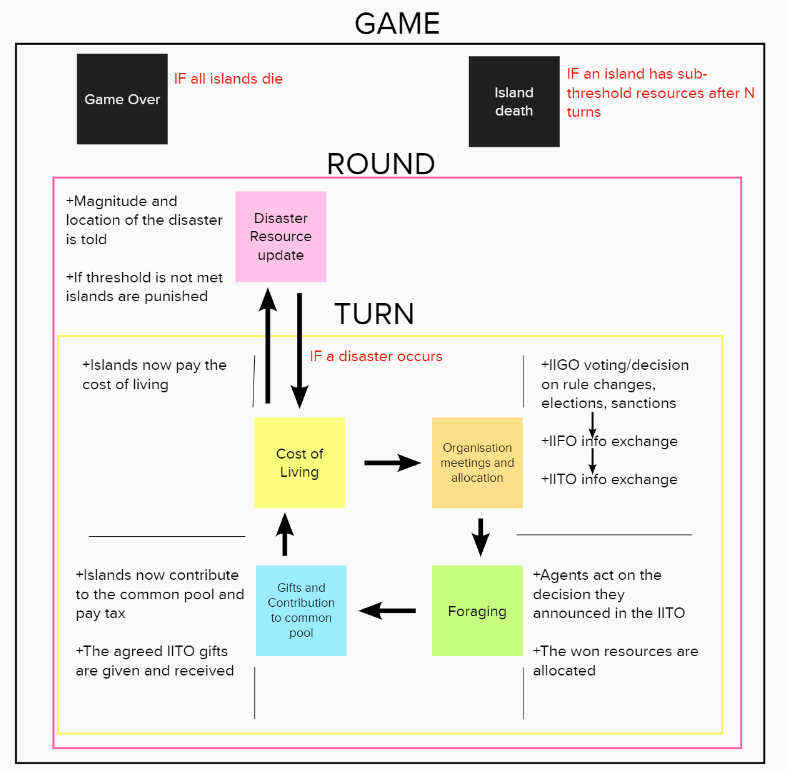
\includegraphics{images/gamespec-flow.png}
    \caption{High Level Game Specification Flow Diagram}
    \label{fig:gamedesign-flow}
\end{figure}
